\chapter{Fundamentals}
\label{ch02:fundamentals}
This chapter covers the technological fundamentals important for the scope of this thesis. The two main technologies covered are Adabas and Kafka, including associated products and software.

\section{Adabas}
\label{ch02:fundamentals:adabas}
This section covers Adabas-related fundamentals. This includes Adabas itself, as well as related products such as the Event Replicator and Target Adapter.

\subsection{Adabas for z/OS}
\label{ch02:fundamentals:adabas:forzos}
Adabas, short for \textbf{Ada}ptable Data\textbf{ba}se \textbf{S}ystem, is a high-performance transactional \ac{DBMS} first launched on a mainframe in 1971. Since then, Adabas has grown to also become available on a variety of systems, including Microsoft Windows, Linux, and other Unix-based platforms. It now includes a range of products, both for the mainframe and \ac{LUW} versions \cite{adabasconcepts}. As the thesis scope is restricted to Adabas on mainframe, the focus of the following fundamentals will be on Adabas for z/OS.
% important adabas terminology for understanding paper
\subsubsection{Adabas Terminology}
To understand Adabas, there are a few fundamental definitions to it that have to be addressed. As a \ac{DBMS}, Adabas can manage multiple databases. Each \textit{database} is a collection of \textit{files}, which are best compared to tables in a relational database. Each file is a "group of related \textit{records}" \cite{adabasconcepts}, which in turn are a "collection of related \textit{fields}" % that make up a complete unit of information???
\cite{adabasconcepts}. Records are comparable to a table row in a relational database, as they usually represent the entire data unit of the represented entity (for example the data of a single employee). The record fields represent the "smallest logical unit of information" \cite{adabasconcepts} and can be grouped into different denormalized data structures.

\subsubsection{Classifying Adabas}
\label{ch02:fundamentals:adabas:forzos:classifying}
% what kind of database is adabas?
Adabas is sometimes called a pre-relational database \cite{ibm_redpaper_key} due to its launch approximately around the same time (or even shortly before) the relational model. Before the relational model, the most common data models were the hierarchical (such as the IBM IMS) and network model \cite{stonebrakerwhatgoesaroundcomesaround}. Adabas is considered a "relational-like \ac{DBMS} with some network features" \cite{adabashybrid}. It has features of the network data model, including support for many-to-many relationships between fields, which are achieved with the multiple field and periodic group structures (discussed further in \ref{ch02:fundamentals:adabas:forzos:datastructures}).

Adabas also contains similar features to a relational data model, such as table-like structures, which can reference one another based on a unique identifier. In the case of Adabas files, the unique identifier is called the \ac{ISN}. Adabas supports both physical coupling of files (similarly to network models) and logical coupling of files \cite{adabasconcepts}. As opposed to the network or hierarchical data model, the coupling relationship is not hierarchical, but instead bidirectional. In the case of physical coupling, files are explicitly linked in the \textit{coupling lists} (managed by the Adabas nucleus) for both files \cite{adabashybrid}. In the case of logical coupling, files can be linked in a query by specifying the common field \cite{adabasconcepts}. % TODO: verify with matthias whether correct!

\subsubsection{The Adabas Nucleus}
% first talk about components such as ASSO, then go into the details
The Adabas nucleus is the core component of the Adabas \ac{DBMS}, containing programs that manage it and allow access to Adabas files. The nucleus uses different database components, each representing a physical disk area, for managing stored data and its retrieval. There are three main components: \textit{ASSO} (Associator), \textit{DATA} (Data Storage), and \textit{WORK} (Work area) \cite{adabasconcepts}.

ASSO is used as an organizational component, storing data structures for data retrieval from the DATA component. It contains elements such as general information about the database, the \ac{FDT} (comparable to a schema) for each file, and the coupling lists mentioned in \ref{ch02:fundamentals:adabas:forzos:classifying} for the coupling of different files in a database \cite{adabasconcepts}. The ASSO also contains \textit{inverted lists} for each file, which is a key feature of Adabas for indexing records by their logical sequence when performing search and read commands \cite{adabashybrid}. In an Adabas file, multiple fields can be labeled \textit{descriptors}. The value of such descriptor fields is then stored in the inverted list with their designated \ac{ISN}s. Thus the list is inverted, as it is ordered by the descriptor values \cite{adabasconcepts}. The ASSO also contains an \textit{address converter} for determining the physical location of each record, called the \ac{RABN}, based on its \ac{ISN}. This allows for physical data independence, as the physical record data can be moved around based on available free space in the DATA component without having to modify the inverted lists \cite{adabashybrid}. 

The DATA component stores the actual record data in a compressed format. It is split up into blocks which are identified by the \ac{RABN}. Each block can contain multiple records depending on their size, as well as some reserved space as padding to allow for the growth of records. Adabas also allows for the physical migration of records in case of growth that the current block cannot support, allowing the database to remain functional and optimized even in case of a growing number (or size) of records \cite{adabasconcepts}.

The WORK component acts as an area for storing information related to transaction routines, two-phase commit processing, and the results of search commands. There exist also further components for specific Adabas utilities, including optional logs. The \ac{CLOG}, for example, is used for keeping information on issued Adabas commands in order to establish an audit trail, while the \ac{PLOG} is used to capture data change in the database, in case there is need for recovery \cite{adabasconcepts}.

\subsubsection{Adabas Data Structures}
\label{ch02:fundamentals:adabas:forzos:datastructures}
% adabas data structures
All of the fields in a file are specified in the \ac{FDT}, which is then used to create the file. Unlike in relational databases, where column order is irrelevant, the order of fields defined in the \ac{FDT} is important and can influence the efficiency of their retrieval \cite{storr1994effizienter}.

"Flat" Adabas fields can have different formats, including packed and unpacked decimals, alphanumeric, and binary. Adabas also has multiple denormalized data structures into which fields can be grouped. It supports groups, multiple fields (MU), and periodic groups (PE), as well as multiple fields in periodic groups \cite{aebi1996reengineering}. A group, as the name suggests, is a grouping of multiple fields under one "parent" name. A group can contain multiple levels (up to 6 levels of nested groups) \cite{storr1994effizienter}. It is recommended to group fields if they are often accessed and are ordered together, allowing faster retrieval by group name \cite{adabasconcepts}. This again highlights the need for fields to be ordered properly in an \ac{FDT}. Multiple fields represent an array of the "flat" Adabas fields, while a periodic group represents multiple instances of a group of fields (an array of a group). Figure \ref{fig:fundamentals:datastructure} shows an example record (without its \ac{ISN}) containing different field types:
\begin{itemize}
    \item Flat fields PERSONNEL\_ID, MARSTAT, SEX
    \item Group field FULLNAME with level 2 sub-fields FIRST\_NAME, NAME, MIDDLE\_NAME
    \item Periodic group field of two occurrences with fields CURRCODE, SALARY, and multiple field BONUS (containing 3 MU occurrences in the first PE occurence, and 2 MU occurrences in the second PE occurrence)
    \item Multiple field LANG with 3 occurrences
\end{itemize}

\begin{figure}[htbp]
 \centering
 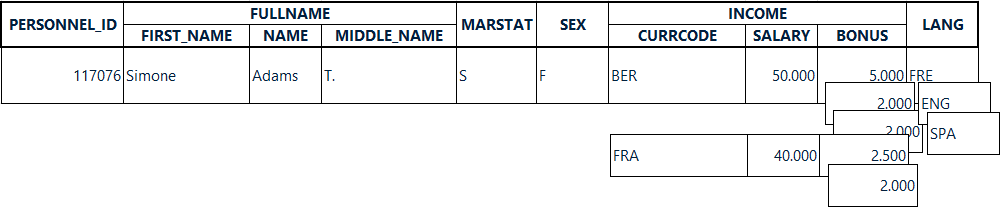
\includegraphics[width=1\textwidth]{chapters/images/datastructures.png}
 \caption[Example structure of a record containing various Adabas data structures]{Example structure of a record containing various Adabas data structures (see \ref{fig:appendix02:adabasstructure} for enlarged version)}
 \label{fig:fundamentals:datastructure}
\end{figure}

\subsubsection{Adabas Transactions}
\label{ch02:fundamentals:adabas:forzos:transactions}
Adabas operates with so-called \textit{logical transactions}: the transaction contains a user-defined \ac{UOW} that must be committed and processed as an atomary \ac{UOW} with the all-or-nothing principle. A transaction has to end either with an \ac{ET} command (in case of success) or with a \ac{BT} command (in case of an error or other issue). If the \ac{BT} command is issued, a rollback is performed of all the updates within that transaction \cite{adabasconcepts}.

% The \ac{REPTOR} (see \ref{ch02:fundamentals:adabas:reptor}) identifies each transaction with its transaction commit time and sequence number (which is relative, as it is always reset when the \ac{REPTOR} restarts). - include in reptor fundamentals
\subsection{Adabas Event Replicator}
\label{ch02:fundamentals:adabas:reptor}
The \ac{REPTOR} was developed by Software GmbH as a replication solution to capture changes in Adabas files. It is made up of multiple components, also hosted on the mainframe, which facilitate the replication of any record modifications processed by the Adabas nucleus \cite{storr2011reptor}.

\begin{figure}[htbp]
 \centering
 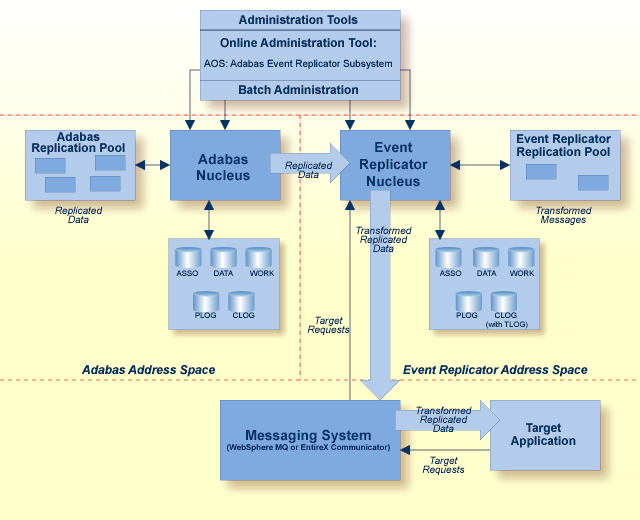
\includegraphics[width=0.8\textwidth]{chapters/images/reptor_architecture.png}
 \caption[Adabas and Event Replicator Components]{Adabas and Event Replicator Components \cite{reptorconcepts}}
 \label{fig:fundamentals:reptorarchitecture}
\end{figure}

As shown in Figure \ref{fig:fundamentals:reptorarchitecture}, any record changes processed by the Adabas nucleus are replicated and stored in the Adabas replication pool until a transaction commit occurs. After the \ac{ET} command, the committed data is copied from the Adabas replication pool, transformed, and saved to the \ac{REPTOR} replication pool. After the transformed transaction messages have been processed by a pre-defined set of rules (called a \textit{subscription}), they are sent to a messaging system\footnote{There are currently two messaging systems supported: the IBM MQ or the EntireX Broker.}. After the replication process is completed and successfully sent to the messaging system, the replicated transaction data is deleted from both replication pools \cite{reptorconcepts}. The target application consuming the message queue can also send \ac{RPC} to the \ac{REPTOR} nucleus through the messaging system, such as requests for status messages. If the messaging system is unavailable or the \ac{REPTOR} replication pool starts to overflow, the overflowing transactions can be written to the \ac{SLOG} file to prevent their loss \cite{storr2011reptor}. The \ac{REPTOR} supports two formats for replicated messages: XML and binary \cite{artconcepts}.

\ac{REPTOR} messages can be classified into four different event types: Delete, Insert, \ac{IS}, and Update. The \ac{IS} event is an event in which the entire current state of the Adabas file is sent \cite{reptorprogrammersref}. This is necessary, for example, when populating the target database for the first time. The \ac{IS} event can be transmitted to the target application using the same messaging system as the other \ac{REPTOR} events. However, there also exists an Adabas utility called ADARIS, which allows the entire \ac{IS} to be split up and written to one or more sequential files. These can then be imported and processed by the target application \cite{reptorconcepts}. This can be quite beneficial, as an \ac{IS} volume can get quite large in enterprise systems with over a million records.

\subsubsection{EntireX Broker}
\label{ch02:fundamentals:adabas:entirex}
The message queue covered in this thesis is the EntireX Broker, as it was already being used internally for development. The EntireX Broker acts as message-oriented middleware, allowing reliable communication with high performance and availability \cite{entirexbrokerintro}. It supports transactional integrity by using units of work\footnote{Not to be confused with the transactional \ac{UOW} from \ref{ch02:fundamentals:adabas:forzos:transactions}.} to group together messages, which are then treated by the Broker as an atomary unit. Message delivery is guaranteed by the receiver application, which must send a COMMIT acknowledgement for each \ac{UOW} received. If a client receives the \ac{UOW} and processes it but does not send a COMMIT message to the Broker, that specific \ac{UOW} can be re-delivered to the message queue, marked as timed out, or processed in some other way based on the broker configuration \cite{entirexbrokeradmin}. This is useful in the case that a client application receives the messages but fails or crashes before it is able to process them fully, preventing a COMMIT message from being sent. In that case, it would be necessary for all the messages within the unprocessed \ac{UOW} to be re-processed by the client application once it is running again.

\subsection{Event Replicator Target Adapter}
\label{ch02:fundamentals:adabas:art}
The Event Replicator Target Adapter (\ac{ART}) is another Software GmbH product that allows the transformation of replicated data into a specified format, to be written to a target application such as a relational database \cite{artconcepts}. Although \ac{ART} was initially created for various relational databases as targets, it supports any custom target which can be developed using the publicly available source code\footnote{\url{https://github.com/SoftwareAG/adabas-user-targets}}. This can include a custom target solution for a data warehouse or a custom Kafka producer.

\ac{ART} can be installed using the Software GmbH installer, which also provides the Administration tool for a graphical user interface and a Replication Monitoring tool to visualize the status of the \ac{REPTOR} \cite{artconcepts}. It can also run headless in a Docker container, with the XML configuration files added manually.

\subsubsection{Schema Transformation}
\label{ch02:fundamentals:adabas:art:schematransformation}
To allow Adabas records to be inserted into a relational database, they first have to be flattened and normalized if they contain any of the aforementioned data structures from \ref{ch02:fundamentals:adabas:forzos:datastructures}. \ac{ART} has a Data Mapping Tool for defining a custom relational schema for the target. There also exists a default transformation \cite{artconcepts}. The following data structures are affected in the default transformation \cite{artconcepts}:
\begin{description}
\item [Group fields]
Group fields are flattened by adding the child fields directly to the root table. In the case of the group field FULLNAME from Figure \ref{fig:fundamentals:datastructure}, the table will contain the fields FIRST\_NAME, NAME, and MIDDLE\_NAME.
\item [Multiple fields]
Each MU field is mapped to a separate relational table, where each value is represented as a separate row with the possibility of tracking the MU index\footnote{An index, or occurrence, indicates the position of the value in the repeating MU or PE field.} as a separate column. The LANG field in Figure \ref{fig:fundamentals:datastructure} is an MU field with three occurrences. Listing \ref{lst:bonusmuquery}  shows how the MU field would be structured in the table. The foreign key constraint is inherited from the root table primary key(s). No primary keys are set in the MU table.
\item[Periodic groups]
Each PE group is also mapped to a separate relational table. Each sub-field in the periodic group is represented by a column in the table. An additional index field is created, composed from the \ac{ISN} and PE field index, which serves as the primary key. The foreign key constraint that references the root table is on the \ac{ISN} field. An example PE field can be seen in listing \ref{lst:bonusmuquery}.

In the case of an MU field in a PE group, a separate table is created with the same logic as a typical MU table, except that an IX2 field is used instead of the IX field to show its nested nature. The aforementioned composed index field is also added to the new MU table with a foreign key constraint referencing the parent PE table. An example MU field in a PE group can be seen in Listing \ref{lst:bonusmupequery}.
% TODO: pk and fk fields of the index, reference listing
\end{description}

In the root table, primary keys are set based on the schema of the Adabas file. If any fields are marked as UQ (unique) in the schema, they are used as the primary keys. If none are specified, the \ac{ISN} is used as the primary key.
\newpage
\begin{lstlisting}[frame=tb,caption={Query result of the MU field LANG in the relational table EMPL\_LANG},label=lst:bonusmuquery]
 ISN | LANG | LANG_IX
-----+------+---------
   1 | FRE  |       1
   1 | ENG  |       2
   1 | SPA  |       3
\end{lstlisting}

\begin{lstlisting}[frame=tb,caption={Query result of the PE field INCOME in the relational table EMPL\_INCOME},label=lst:incomepequery]
  ISN   | INCOME_INDEX | ISN_INCOME_INDEX | CURRCODE | SALARY
--------+--------------+------------------+----------+--------
      1 |            1 |      1_1         | BER      |  50000
      1 |            2 |      1_2         | FRA      |  40000
\end{lstlisting}
% \newpage
\begin{lstlisting}[frame=tb,caption={Query result of the MU field BONUS in the PE field INCOME in the relational table EMPL\_INCOME\_BONUS},label=lst:bonusmupequery]
 ISN_INCOME_INDEX | BONUS | BONUS_IX2
------------------+-------+-----------
 1_1              |  5000 |         1
 1_1              |  2000 |         2
 1_1              |  2000 |         3
 1_2              |  2500 |         1
 1_2              |  2000 |         2
\end{lstlisting}


\subsubsection{Drawbacks of the Target Adapter}
\label{ch02:fundamentals:adabas:art:limitations}
There have been some performance concerns noted both by clients and developers when using \ac{ART} to replicate to a relational database. Possible causes could be the fact that \ac{ART} for Adabas on mainframe only supports messages in XML format, which can negatively impact performance \cite{nicola2003xml}. Another cause is speculated to be the lack of parallelism when replicating to relational databases. The only parallel processing that is supported by \ac{ART} is when loading the \ac{IS} using multiple ADARIS-generated files. This can be achieved by running multiple instances of \ac{ART}, where each instance processes one of the generated ADARIS files.

\section{The Kafka Ecosystem}
\label{ch02:fundamentals:apachekafkaandkafkaconnect}
This section covers fundamentals related to the Kafka ecosystem. It introduces Apache Kafka, as well as the Kafka Connect framework and Schema Registry.
\subsection{Apache Kafka}
\label{ch02:fundamentals:apachekafkaandkafkaconnect:apachekafka}
Apache Kafka is a distributed event streaming platform developed by LinkedIn and currently managed by the Apache Foundation, offering high-throughput and fault-tolerant data processing. A behemoth of streaming possibilities, it runs as a cluster of one or more machines called \textit{brokers}. They organize incoming messages (also called Kafka events) in \textit{topics}, which can be asynchronously published to with \textit{producers} and consumed from by \textit{consumers} \cite{peddireddystreamliningprocessingkafka}. To facilitate scalability and parallel processing, a topic can be divided into multiple \textit{partitions}. Message order is only guaranteed for a single partition, so that if two messages are added in a consequent order to two different partitions, they will not necessarily be consumed in the same order. Messages are organized by a sequential \textit{offset} number in each partition \cite{thein2014apache}.

There are different strategies for determining to what partition a message is assigned to. The default strategy involves hashing the message key to map it to a partition. If the key is null, either the "sticky partition" strategy is used (where messages are produced to one partition until a certain batch size is achieved) or the round-robin strategy. Kafka also supports writing custom partitioners to implement a specialized partitioning strategy  \cite{kafkadocumentation}.

Partitions can be stored on different brokers running in the same cluster, so that client applications can consume from and produce to different brokers, improving load balancing and scalability. Partitions can also be replicated to additional brokers (the number of replicas is determined by the \textit{replication factor} configuration), improving Kafka's fault tolerance \cite{thein2014apache}. Each partition gets assigned a broker leader, with that broker then being responsible for the reads and writes to that partition. The rest of the brokers act as "followers" of that partition and have the ability to replicate it, based on the cluster configuration \cite{petrescukafkaraft}. These brokers then maintain the so-called \ac{ISR} of the partition. This mechanism guarantees message consistency and fault tolerance for the consumer, as a message is only ever truly considered committed (and available to a consumer) if the specified number of \ac{ISR} are synchronized with the leader partition \cite{kafkadocumentation}.

Kafka provides three possible message delivery guarantees, using the message offset to track a consumer's position in a partition: at most once, the default at least once, and exactly once \cite{kafkadocumentation}. Kafka uses the notion of \textit{consumer groups}, where the message offset position is tracked for each group instead of the individual consumer. If there are multiple consumers in one consumer group, each message is typically delivered to only one of them \cite{kreps2011kafka}.

Older versions of Kafka rely on Zookeeper, a separate service used for organizing brokers and consumers, keeping track of consumer groups and their progress, and rebalancing consumers in case of consumer load or broker number change \cite{kreps2011kafka}. It facilitates leader election in the Kafka cluster, so that a single controller can be chosen among the brokers to make cluster-relevant decisions. One such decision is assigning partition leader roles. However, as of Kafka version 3.5, Zookeeper is marked as deprecated and planned for removal \cite{kafkadocumentation}. Instead, Kafka now supports running in KRaft mode, based on the Raft concensus algorithm \cite{ongaroraft2014search}. In KRaft mode, Kafka nodes can act as brokers, controllers, or both, removing the need for Zookeeper. The Kafka nodes assigned the controller role participate in a quorum to elect a controller leader \cite{kafkadocumentation}.

It is important to note that Kafka is not intended to be used as a permanent storage for events. Instead, it has a configurable retention period (specified in time and/or byte size), after which messages are deleted from the brokers. This allows for a certain "grace period", in case older offsets need to be consumed again, without keeping old and unnecessary data for too long \cite{kreps2011kafka}.

\subsection{Kafka Connect}
\label{ch02:fundamentals:apachekafkaandkafkaconnect:kafkaconnect}
Kafka Connect is an open-source framework developed for Apache Kafka to allow for reliable and scalable data integration between Kafka and external systems such as databases. The Apache Foundation offers publicly available \ac{APIs} for implementing source connectors (to produce data to Kafka) and sink connectors (to consume from Kafka and write to external systems) \cite{kafkadocumentation}. Some companies such as Confluent provide already existing connectors, such as the \ac{JDBC} source and sink connectors\footnote{\url{https://github.com/confluentinc/kafka-connect-jdbc}}.

While it is possible to not use Kafka Connect and instead write producers as part of the source system to capture any changes, tests performed by \cite{srijithkafkaconnectperformance} have shown that the traditional publish-subscribe model can perform worse than a Kafka Connect pipeline. Furthermore, \cite{maison2023kafkaconnect} identified the number of threads reserved for producer operations in the source system as a possible performance bottleneck. This is improved with Kafka connectors, which can be scaled independently of the source system, showing positive performance results in both papers.

Kafka Connect has two modes: standalone and distributed. In standalone mode, the Kafka Connect setup consists of a single host node (\textit{worker}) that can run multiple tasks. The task is the component that actually performs the data processing and transfer in the connector and is assigned work by the connector \cite{kafkadocumentation}. In distributed mode, the setup consists of multiple workers running as a Connect cluster. The workers distribute the tasks between themselves for a more equal workload, as well as take over tasks from a crashed or unavailable worker \cite{maison2023kafkaconnect}. It is also possible to run multiple connectors (for example source and sink) in the same Connect cluster (see Figure \ref{fig:fundamentals:kafkaconnectexample}). When running in distributed mode, the offset and configuration data necessary to run the connectors is stored in internal Kafka topics \cite{kafkadocumentation}.

\begin{figure}[htbp]
 \centering
 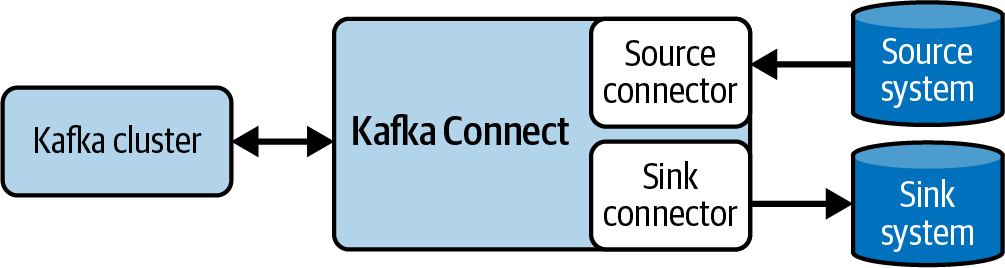
\includegraphics[width=0.6\textwidth]{chapters/images/kafkaconnectexample.png}
 \caption[Visualization of Kafka Connect with Sink and Source Connector]{Visualization of Kafka Connect with Sink and Source Connector \cite{maison2023kafkaconnect}}
 \label{fig:fundamentals:kafkaconnectexample}
\end{figure}

The number of tasks run by each connector is determined by the \textit{tasks.max} configuration. The number of active tasks in source connectors is also typically constrained by the number of source partitions, if the source is partitioned at all. Not to be confused with topic partitions, source partitions are used for splitting up the source into logical groups. For example, partitioning a relational database source can mean to treat each table as a separate source partition. Each source partition can typically be assigned a single task to process it (meanwhile, a task can process multiple source partitions). This allows the source connector to parallelize the processing of the source \cite{maison2023kafkaconnect}.

Figure \ref{fig:fundamentals:kafkaconnectarchitecture} shows the possible architecture of a source connector running in distributed mode with two Connect workers. There are 4 tasks running and 5 source partitions, so the first task gets assigned two of the source partitions. As per the default partitioning strategy, each event processed by the task is assigned a message key before it gets produced to Kafka. This key is then used to determine the topic partition that the message is assigned to.

\begin{figure}[htbp]
 \centering
 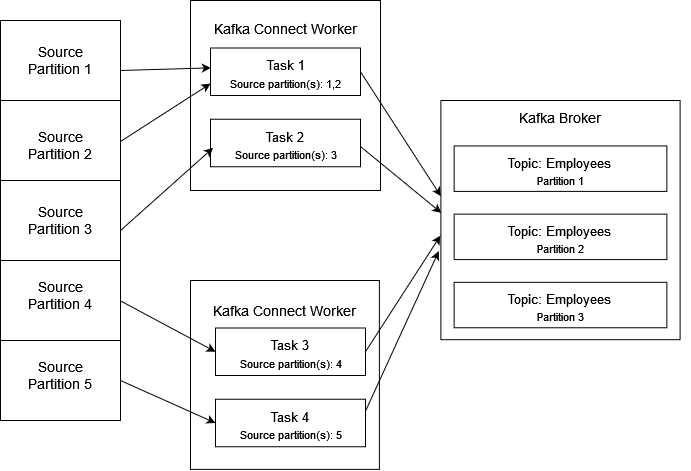
\includegraphics[width=0.8\textwidth]{chapters/images/kafka connect architecture enlarged.drawio.png}
 \caption[Example Architecture of a Kafka Source Connector in Distributed Mode]{Example Architecture of a Kafka Source Connector in Distributed Mode (see \ref{fig:appendix02:kafkaconnectarchitecture} for enlarged version)}
 \label{fig:fundamentals:kafkaconnectarchitecture}
\end{figure}

% \subsection{Transactionality in Kafka}

\subsection{Schema Registry}
The schema registry is a component that is not native to Apache Kafka, but is a third-party addition. It is run as a separate service, and allows for the creation, management, and evolution tracking of message schemas. With it, the producer and consumer can establish a "data contract", so that events produced to Kafka can be deserialized and read properly \cite{kreps2011kafka}. This is especially useful as Kafka supports different serialization formats such as JSON, Protobuf, and Avro \cite{kafkadocumentation}.
% Although the same can be accomplished without the registry by sending the message schema with every event, the message size increase and resulting performance impact should be taken into account.

% \section{Database Replication}
% \label{ch02:fundamentals:databasereplication}

% \subsection{Relational Databases}
% \label{ch02:fundamentals:databasereplication:relationaldatabases}

% \subsection{Schema Transformation}
% \label{ch02:fundamentals:databasereplication:schematransformation}